\documentclass{article}
\usepackage {inputenc, fullpage, listings, amsmath, graphicx}

\parindent 0pt

\title{%
   ECE 458 (Spring 2022) Assignment 4 \\
   \large Alex Holland V00}
    
\date{}

\begin{document}

\maketitle

{\bf Question 1}\\
A control plane that is based on logically centralized control means that it knows all the routing and forwarding tables in the routers of the network. The data plane consists of different network switches which can execute "Match Plus Action" rules in the flow tables. Whereas, the control plane is made up of various servers and software that are handled by the switch's flow table. Thus the data plane and the control plane are implemented in separate devices.

\bigskip
{\bf Question 2}\\
The autonomous system's intra-routing algorithm is used to determine the cheapest path from each internal router to the gateway. It is not necessary that every autonomous system use the same intra-AS routing algorithm. This is because each autonomous system has a specific administrative autonomy for routing within an autonomous system.

\bigskip
{\bf Question 3}\\
Similarities:
Both link-state and distance-vector routing algorithms:
\begin{itemize}
    \item Determines the least-cost path between a source and destination.
    \item Finds the best path from a source to destination router from a set of routers and their connecting links.
\end{itemize}

Differences:
\begin{itemize}
    \item Link-state algorithm take the network topology and link costs as input, while the distance-vector algorithm takes all the associated costs with the current node to all of its neighbors.
    \item Distance-vector routing is based on the Bellman-Ford algorithm while link-state is based on Dijkstra's algorithm.
    \item More Memory space and CPU utilization is generally required for distance-vector algorithm compared to link-state algorithm.
\end{itemize}

\bigskip
{\bf Question 4}\\
The NEXT-HOP is the router interface that initiates the AS-PATH. The NEXT-HOP attribute is required for establishing a connection between the Inter-AS and Intra-AS routing protocols. The IP address of the first router in the advertised path, which is the advertisement received by the external AS to a specific prefix, is specified by the NEXT-HOP attribute. The AS-PATH attribute is used by the routers to identify and avoid looping advertising. When the router determines that the AS is already in the list, the advertisement is refused. This list (AS-PATH attribute) holds the autonomous system number that the router has traversed.


\pagebreak
{\bf Question 5}\\
Definitions of the following terms in the context of SNMP:\\

Managing Server - An application in the network used to govern the devices in the network by controlling the collection, processing, analysis, and display of network management information.\\

Managed Device - Piece of network-connected equipment such as a switch, modem, host, or router which is included on a managed network.\\

Network Management Agent - Software that runs in a managed device's that connects with the managing server and performs action on the managed device under the managing server's control. \\

MTB - Management Information Base is a collection of information about all the managed object which is within the managed device.

\bigskip
{\bf Question 6}
\begin{center}
    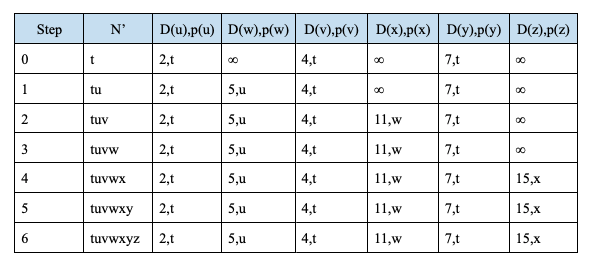
\includegraphics[width=1\textwidth]{6-1.png}
\end{center}

\begin{center}
    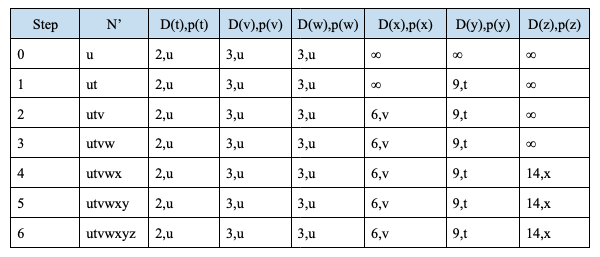
\includegraphics[width=1\textwidth]{6-2.png}
\end{center}

\begin{center}
    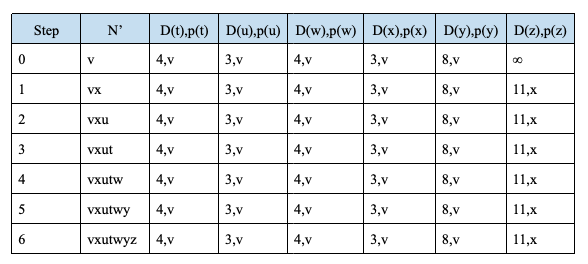
\includegraphics[width=1\textwidth]{6-3.png}
\end{center}

\begin{center}
    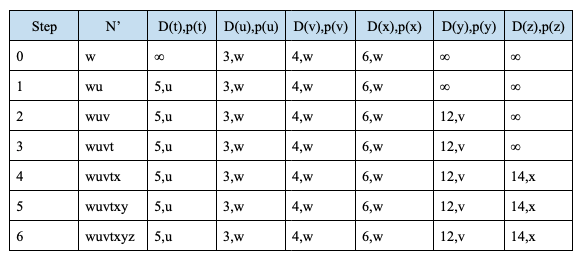
\includegraphics[width=1\textwidth]{6-4.png}
\end{center}

\begin{center}
    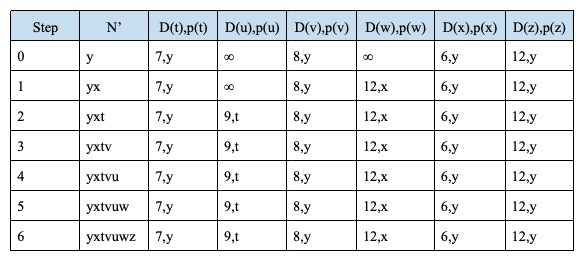
\includegraphics[width=1\textwidth]{6-5.png}
\end{center}

\begin{center}
    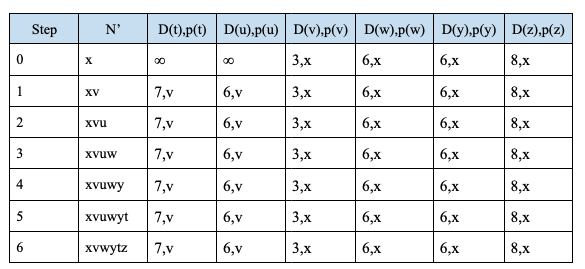
\includegraphics[width=1\textwidth]{6-6.png}
\end{center}

\begin{center}
    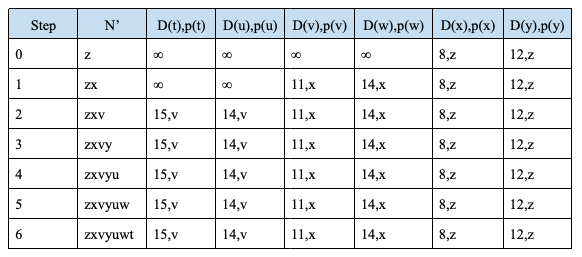
\includegraphics[width=1\textwidth]{6-7.png}
\end{center}

{\bf Question 7}\\
Consider the distance vector algorithm, we want to show the table entries at node $z$.\\

At first, node $z$ will know the cost of only it's direct neighbors:
\begin{center}
    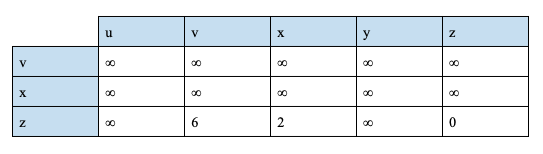
\includegraphics[width=1\textwidth]{7-1.png}
\end{center}

After exploring node $v$ and $x$ we can check nodes $u$ and $y$ and there their new paths. Additionally, We can update the table if any of the paths that are cheaper:
\begin{center}
    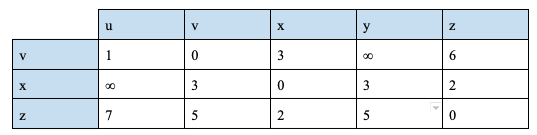
\includegraphics[width=1\textwidth]{7-2.png}
\end{center}

After exploring all the nodes in the network we can determine all optimal routes. Thus the final table entries at node $z$ is:
\begin{center}
    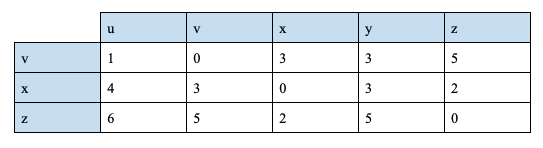
\includegraphics[width=1\textwidth]{7-3.png}
\end{center}

{\bf Question 8}\\
four active nodes—nodes A, B, C and D are competing for access to a channel using slotted ALOHA. We will assume that each node has an infinite number of packets to send. Let the probability that A, V, C, and D succeeds to transmit in each slot be represented as $p(A), p(B), p(C),$ and $p(D)$.

{\bf a)}\\
The probability that node A succeeds for the first time in slot 5 can be represented as:\\
\begin{equation*}
\begin{split}
    p(A) &= p(A \; succeeds \; in \; a \; slot)\\
    & (1-p(A))^4 p(A)\\
    p(A) &= p(A \; transmits \; and \; other \; nodes \; don't)\\
    &= p(1-p)(1-p)(1-p)\\
    &= p(1-p)^3\\
    p(A) &= p(A succeeds first time in slot 5)\\ 
    p(A) &= p(1-p(A))^4p(A)\\
    &= (1-p(1-p)^3)^4 \times p(1-p)^3\\
\end{split}
\end{equation*} 

\smallskip
{\bf b)}\\
the probability that some node (either A, B, C or D) succeeds in slot 4 can be represented as:
\begin{equation*}
\begin{split}
    p(A) = p(1-p)^{4-1}=p(1-p)^3\\
    p(B) = p(1-p)^{4-1}=p(1-p)^3\\
    p(C) = p(1-p)^{4-1}=p(1-p)^3\\
    p(D) = p(1-p)^{4-1}=p(1-p)^3\\
\end{split}
\end{equation*} 
Since these events are mutually exclusive the probability that either A, B, C or D succeeds is $4p(1-p)^3$.

\smallskip
{\bf c)}\\
the probability that the first success occurs in slot 3 can be represented as:
\begin{equation*}
\begin{split}
    p(slot \; 3 \; success) &= 4p(1-p)^3\\
    p(slot \; 3 \; no \; success) &= 1-4p(1-p)^3\\
    p(slot \; 3 \; first \; success) &= p(slot \; 3 \; success) \times p(slot \; 3 \; no \; success)\\
    p(slot \; 3 \; first \; success) &= (1-4p(1-p)^3) \times 4p(1-p)^3
\end{split}
\end{equation*} 

\smallskip
{\bf d)}\\
\begin{equation*}
\begin{split}
    efficiency &= p(slot \; success)\\
    &= 4p(1-p)^3
\end{split}
\end{equation*} 

{\bf Question 9}\\
To determine $R$ we will use Cyclic Redundancy Check The polynomial expression of $G$ is $(x^4 \times 1) +  (x^3 \times 0) + (x^2 \times 0) + (x^1 \times 1) + (x^0 \times 1) = x^4+x^1+1$. So $r=4$, and $D+r=1010101010 \; 0000$. Now we can divide $D+r$ by $G$:
\begin{center}
    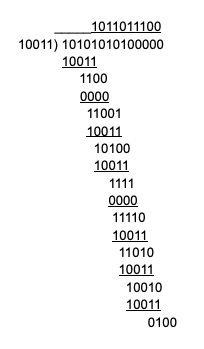
\includegraphics[width=0.28\textwidth]{8.png}
\end{center}
We get that the value of $R=0100$.

\bigskip
{\bf Question 10}\\
If the propagation delay between the two nodes is denoted as $d_{prop}<L/R$ then there will be a collision since while a node is transmitting, it will begin receiving the packet from the other node. 

\end{document}

